\documentclass[10pt,twocolumn]{article}
\usepackage[latin1]{inputenc}
\usepackage{amsfonts}
\usepackage{amssymb}
\usepackage{graphicx}
\usepackage{hyperref}
\usepackage{karnaugh-map}
\usepackage[cmex10]{amsmath}
\usepackage{array}
\usepackage{booktabs}
\usepackage[margin=0.5in]{geometry}
\usetikzlibrary[karnaugh]\usetikzlibrary{arrows,shapes.gates.logic.US,shapes.gates.logic.IEC,calc}

\title{\textbf{ARM Assignment}}
\author{B.Sai Sindhu}
\date{March 2023}
\begin{document}
\maketitle
\section{problem}
In the ciruit X and Y are digital inputs, Z is digital output.The equivalent circuit is the logic implementation of XOR Gate.
\begin{figure}[h]
    \centering
    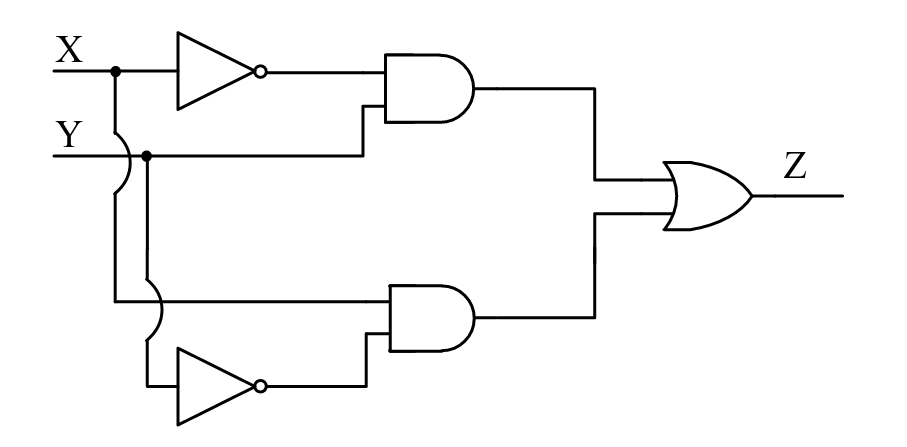
\includegraphics[scale=0.2]{xor.png}
    \caption{Z=X!Y+!XY}
    %\caption{Circuit}
    \label{fig:circuit}
\end{figure}

\section{solution}
    %\caption
    \begin{center}
    	${\boldsymbol{Z}=\boldsymbol{X}\boldsymbol{!Y}+\boldsymbol{!X}\boldsymbol{Y}}$
    \end{center}
    
    %\caption{circuit}
\section{Description}
\large
Given is a boolean expression with three different variables implying that three inputs are to be given for the circuit,in addition to that we have some mathematical operations, apostrophe and dot operators. \vspace{2mm} 
\\ These symbols are nothing but the logic gates
represting AND, OR, NOT gates for symbols "\textbf{.}", "\textbf{+}", " \textbf{'} " respectively. \vspace{2mm}
\\ So, for the given expression 5 distinct logic gates are to be connected using the four inputs in accordance with the boolean expression to excute the logic in pratice.
\section{Procedure}
\raggedright 1.After executing the following code using make, a binary file is generated with .bin extension in the output directory. \vspace{2mm} \\ 
%\centering \underline{\href{https://github.com/BoleManideep/FWC_module1/tree/main/Assignments/assembly/codes}{"Code"}} \\ \vspace{2mm} 
\raggedright 2.Now from the termux, using scp protocol, send the generated bin file to the laptop. \\ \vspace{2mm}
\raggedright 3.There we are supposed to flash the .bin file into the ARM through the terminal.\\ \vspace{2mm}
\raggedright 4.After flashing, reset the Vaman board.\\ \vspace{2mm}
\raggedright 5.Make connections between the LED and ARM board using jumper wires. \\ \vspace{2mm}
\raggedright 6.Now check the output with reference to the truth table present above.

\section{Conclusion}
Hence implemented the given circuit and boolean expression  after verifying it's functionality using ARM.\\
The below code realizes the Boolean logic expression for given 
circuit.
\begin{center}
\fbox{\parbox{8.5cm}{\url{https:https://github.com/sindhu023/FWC/blob/main/arm/src/main.c}}}
\end{center}
\end{document}

